\Chapter{Gazdasági háttér}
A kereskedelem szerves része az életünknek már az ősidőktől fogva. Alapvető minden társadalomban, hogy áruért, szolgáltatásért valamilyen ellenértékkel szolgáljunk. Régen még nem volt jelen a pénz, mint fizetőeszköz, körülbelül az i.e. 7. század elejétől kezdődött el a felhasználásuk. Ekkoriban a tereken, piacutcákon árusították termékeiket az árusok. Innen ered a piac szó, olaszul piazza, amely térséget jelent.

\Section{Piac}
A piac az eladók és vevők cserekapcsolatainak összessége, az eladók és vevők
kölcsönhatásait fejezi ki; elemei közé tartozik többek között a kereslet, kínálat, ár és jövedelem. A vásárlók és az eladók a piacon lépnek interakcióba egymással, a vevők szükségletei az eladók kínálataiból kielégítésre kerülnek. A piacnak többféle formája létezik, melyeket a javak fajtája különböztet meg. Ezek közül, hogy párat említsek, létezik az
\begin{itemize}
  \item árupiac, ahol olyan termékekbe fektethetünk, mint például az olaj, arany, kávé,
  \item a munkaerőpiac, ahol a munkát keresők (eladó) és a munkaerőt kereső (vevő) igénye találkozik,
  \item és a tőkepiac, ami a befektetések, értékpapírok piaca \cite{kozgaz}.
\end{itemize}

\Section{Tőzsde}
A tőzsde egy nyilvános, központosított piac, ahol többek között az értékpapír kereskedelem történik. A tőzsde a másodlagos piaca az értékpapíroknak, ahol a befektetők között történik a tranzakciók lebonyolítása. Ezt úgy kell elképzelni, hogy egy vállalat kibocsát értékpapírokat, ezzel egyidőben az első tulajdonosukhoz kerülnek, és ha úgy dönt az új tulajdonos, hogy ezeket eladná, akkor ezt a másodlagos piacon teszi meg. Mivel ezek az ügyletek bonyolultak, illetve szigorú eljárási szabályokat alkalmaznak, ezért egy befektetési szolgáltatón keresztül kell ezeket lebonyolítani, ezeket brókercégeknek hívjuk \cite{penziranytu}.

\subsection{Részvény}
Az értékpapír kereskedelem egyik lehetősége a részvényekkel történő adás-vétel. A részvény tulajdonképpen egy vállalat által kibocsátott értékpapír, mely tulajdonjogot testesít meg. Ahhoz, hogy részvényt tudjunk vásárolni, szükség van egy értékpapír számlára, amelyet egy brókercégnél szükséges nyitni. Ezután a brókercégen keresztül lehetőség nyílik a szimpatikus vállalatok részvényeinek megvásárlására. Általában egy online felületen történnek ezek a tranzakciók. A részvényekből kétféleképpen is lehet jövedelemre szert tenni: vagy osztalék kifizetésből, vagy az árfolyamnyereségből.
\begin{figure}[ht]
\centering
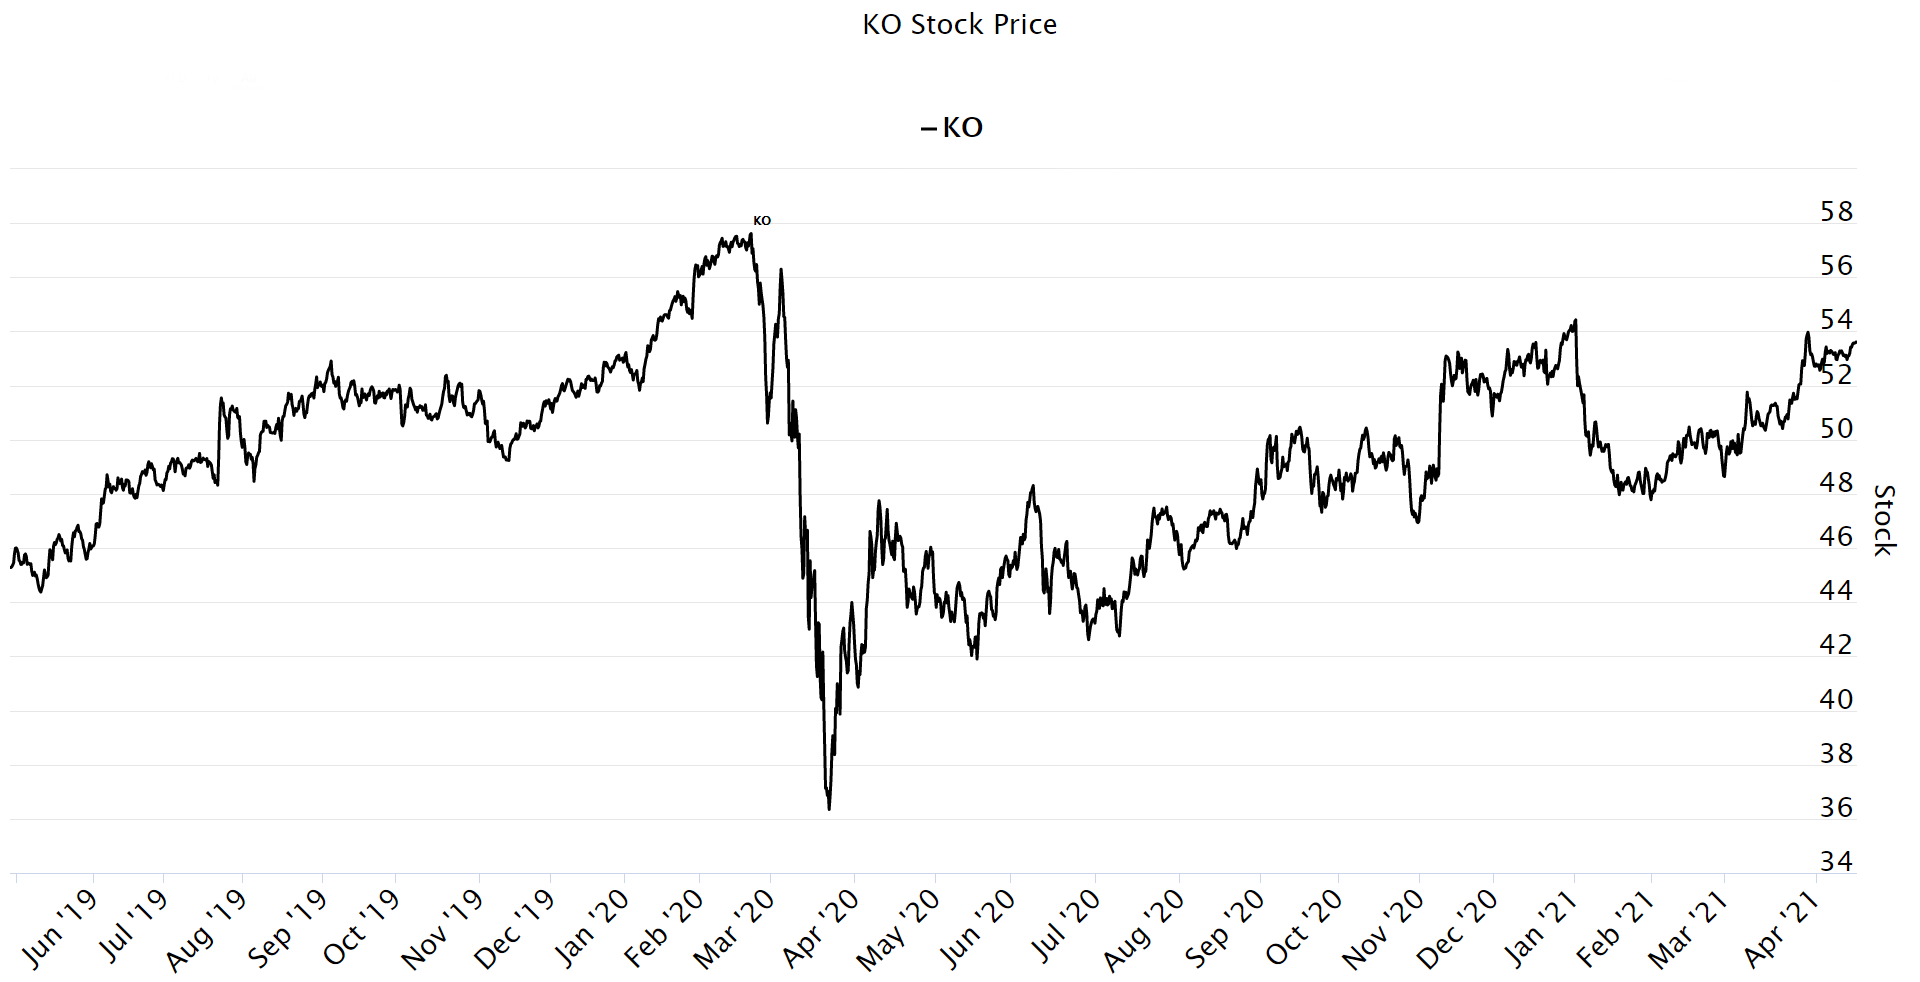
\includegraphics[scale=0.22]{images/KO_stock.png}
\caption{A Coca-Cola részvény záróárai.}
\label{fig:PM}
\end{figure}

\subsection{Osztalék}
Az osztalék a vállalat által megtermelt profitnak az a része, amit kifizet a tulajdonosai részére. Egy vállalat működése akkor hatékony, ha teljesülnek a rövid- és hosszútávú nyereségkövetelmények, köztük a kvázi költségek is. Ekkor a többletét kifizetheti a tulajdonosai részére osztalék formában, azonban ez egyáltalán nem kötelező. Ezért érdemes olyan vállalatot kiválasztani, amely bizonyította már az osztalékfizetési szándékát, mint például a Coca-Cola.
\begin{figure}[ht]
\centering
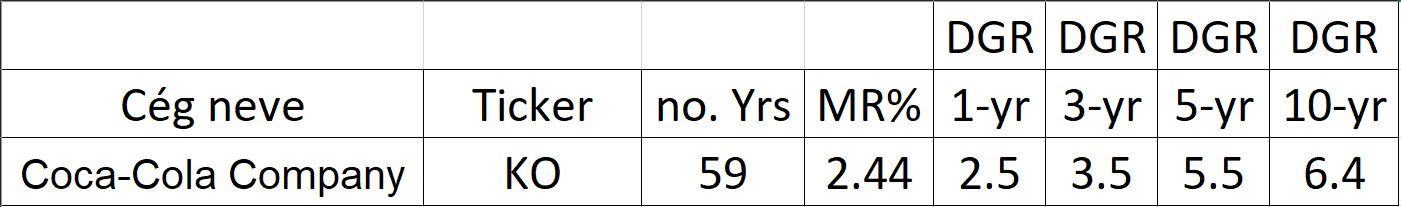
\includegraphics[scale=0.22]{images/coca.png}
\caption{A Coca-Cola osztalékfizetési összefoglalója \cite{dripinvesting}.}
\label{fig:coca}
\end{figure}

\noindent A táblázatban látható adatok jelentése a következő:
\begin{itemize}
  \item Ticker a cég egyedi azonosítója, mely a tőzsdén azonosítja,
  \item no. Yrs oszlop mutatja, hogy hány éven keresztül emelte az osztalékát,
  \item MR\% mutatja a legfrissebb emelés mértékét,
  \item DGR oszlopok pedig azt írják le, hogy az alattuk jelzett időtávokon átlagosan mennyivel emelkedett az osztalék.
\end{itemize}
Érdemes megnézni egy vállalat osztalékfizetési szokásait vásárlás előtt. Az a cég remek célpont nagyvonalakban, amely folyamatosan emeli az osztalékát, az osztalékfizetési trendjét nézve nem található csökkenés, és a DGR mutatói nem romlanak \cite{solyomi2017}.

\subsection{Árfolyamkülönbség alapú profitálás}
A másik lehetséges módja a pénzkeresésnek az, ha olcsón megvesszük a részvényt, majd drágábban eladjuk, számításba véve a kötelező adózási feltételeket. A szakdolgozatom fő célja, hogy megtaláljam azokat az időpontokat, amikor érdemes vásárolni, illetve eladni.
\begin{figure}[ht]
\centering
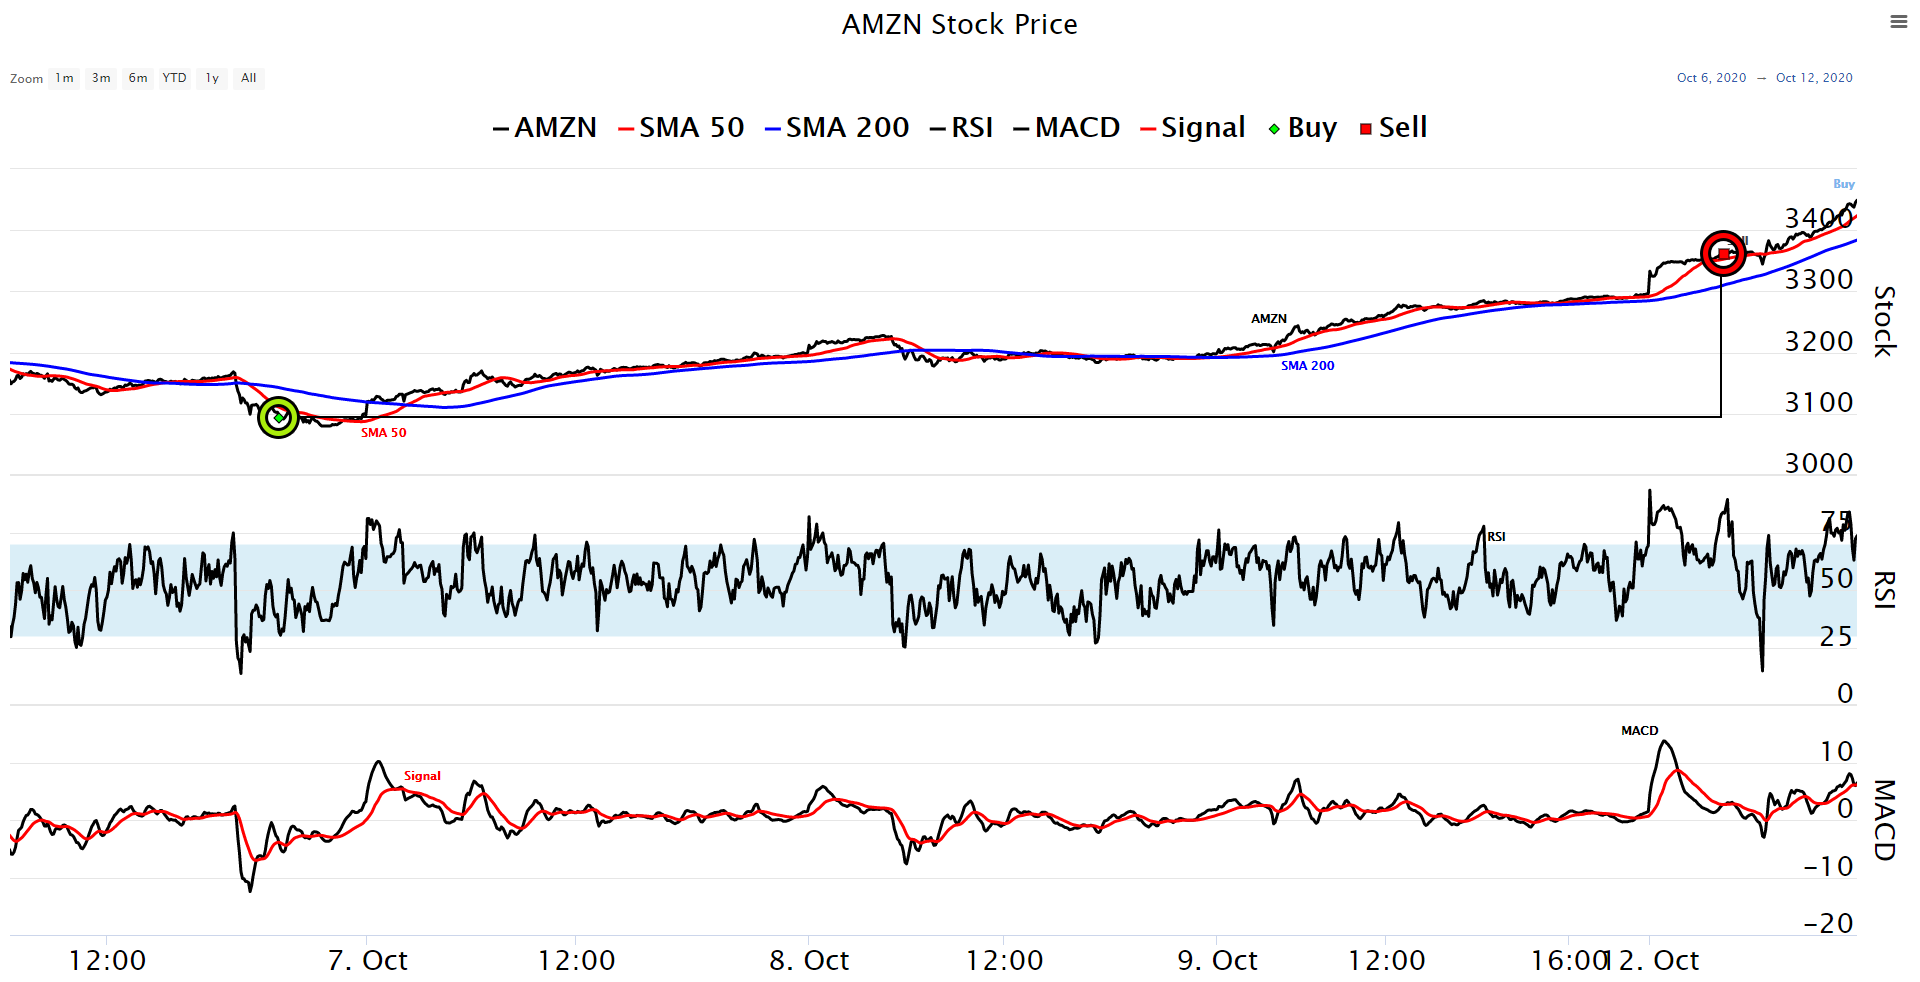
\includegraphics[width=\textwidth]{images/AMZN_profit.png}
\caption{Az Amazon vállalat részvényén történt árfolyamnyereség.}
\label{fig:AMZN_profit}
\end{figure}
Az alábbi ábrán az algoritmus 269\$ profitot termelt részvényenként, amely elég szép eredménynek tekinthető. Ezt a profitot később vissza tudja forgatni részvény vásárlásba, azonban ez egyúttal a kockázatot is növeli.

A következő alfejezetekben részletesebben bemutatom a kereskedéshez használt indikátorokat, illetve azokat a jellemzőiket, amelyek segítenek eldönteni, hogy érdemes-e vásárolni a részvényből vagy sem. Ezek az indikátorok közismertek, és előszeretettel használják a befektetők a technikai analízis során. Mindegyik indikátornál más és más fogja jelenteni a vásárlási és eladási jelzést, ezekre bővebben kitérek minden indikátor esetében.

\Section{Simple Moving Average (SMA)}
Az SMA, avagy az egyszerű mozgóátlag a legkönnyebben használható indikátor, tulajdonképpen egy tartomány átlagát kell venni a kiszámításához.
$$
\text{SMA} = \frac{A_1 + A_2 + \ldots + A_n}{n},
$$
ahol \\
\hspace*{9mm} \makebox[5mm]{$A_i$:} részvény záróárai, \\
\hspace*{9mm} \makebox[5mm]{$n$:} a vizsgált periódus.

\noindent Az SMA-t arra használjuk, hogy megnézzük milyen irányba mozog a trend. A 200 periódusú SMA-t szokás használni hosszútávú trend vizsgálatára, az 50 periódusút pedig középtávúnak tekintjük. Általában arra használjuk, hogy az árakat, illetve a technikai indikátorokat kisimítsuk, viszont meg kell találni egy arany középutat, hisz minél nagyobb a periódus, annál nagyobb a simítás mellett a késése is a jelzésnek.

\begin{figure}[ht]
\centering
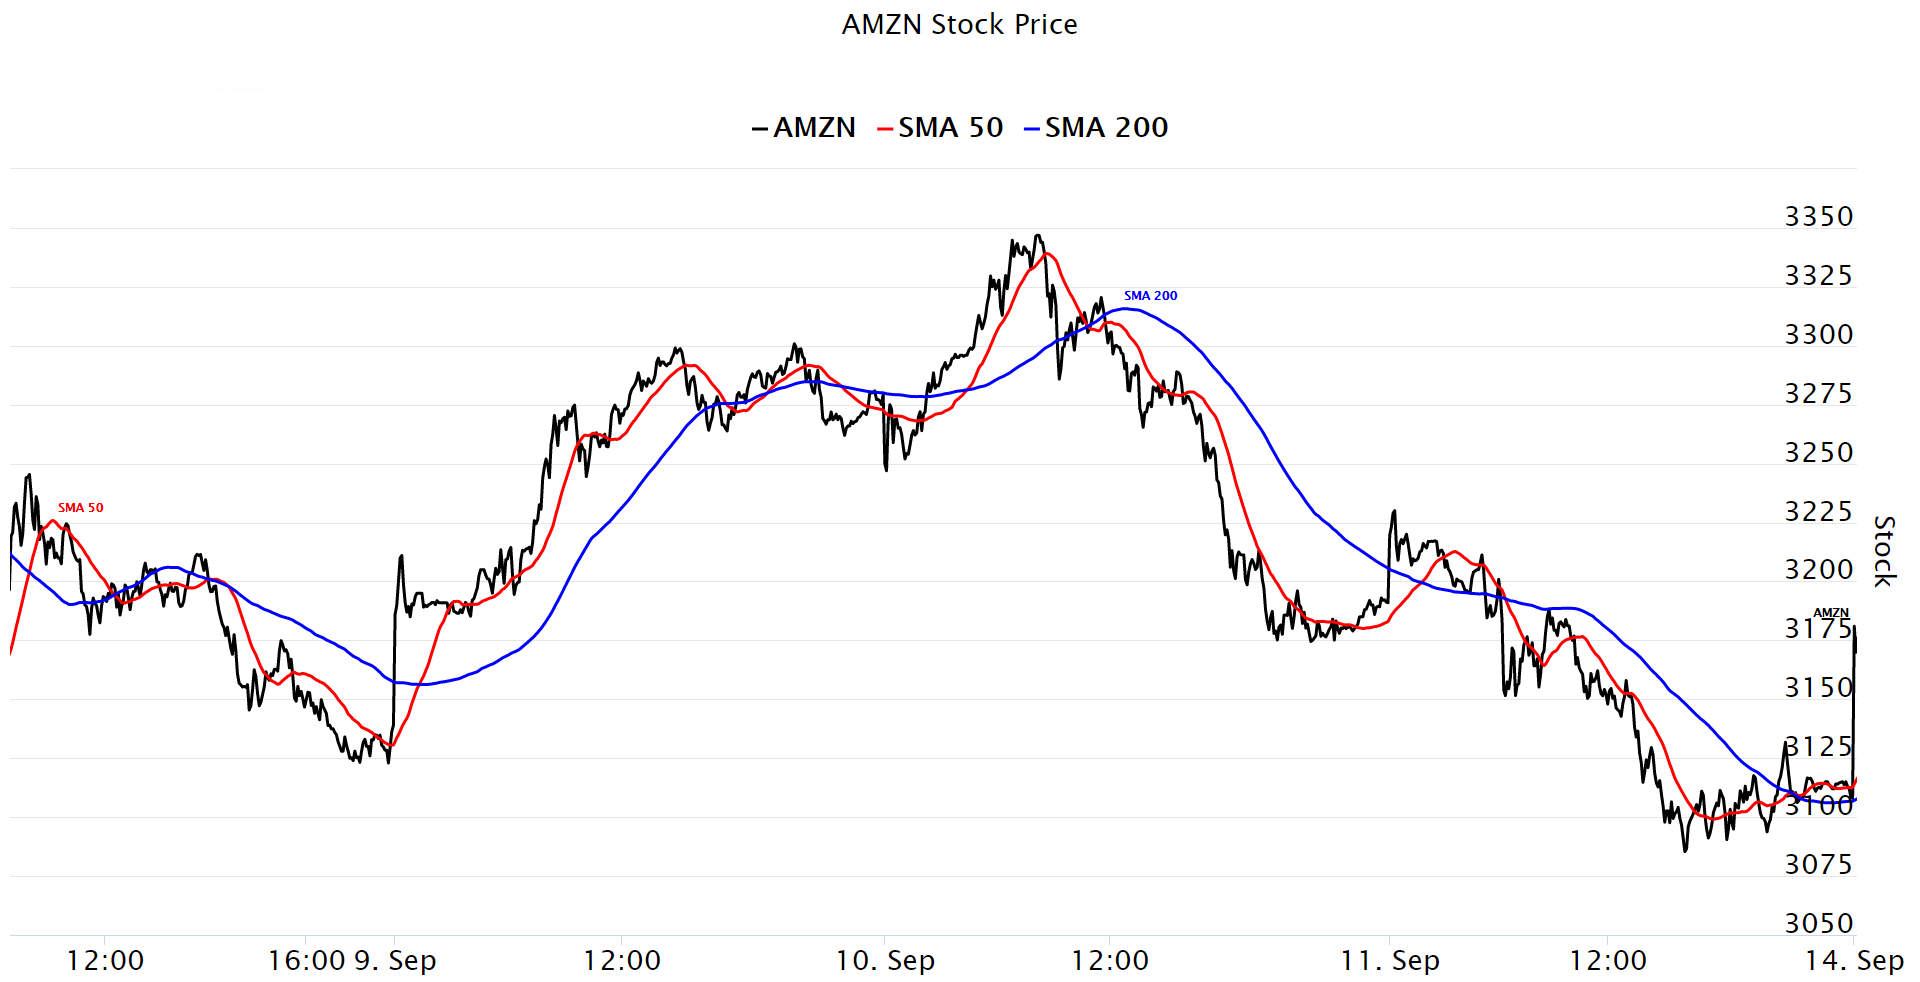
\includegraphics[width=\textwidth]{images/trend.png}
\caption{Az 50 napos és a 200 napos mozgóátlag grafikonja.}
\label{fig:trend}
\end{figure}

Az ábrán látható, hogy az 50 periódusú SMA mennyivel gyorsabban leköveti az árfolyam mozgását, mint a 200 periódusú társa. Az 50 periódusú és a 200 periódusú SMA együtt nézve felhasználható szignálként.

\subsection{Aranykereszt}
Amikor a rövid periódusú SMA alulról keresztezi a hosszabb periódusút, akkor ezt egy vásárlási jelzésként értelmezhetjük. Ezt a találkozási pontot aranykeresztnek nevezzük. Azt mondhatjuk, hogy az aranykereszt egy megbízható jelzés, azonban a kereskedők más indikátorokkal is meg szokták erősíteni a jelzést.

\subsection{Halálkereszt}
Halálkeresztről akkor beszélünk, ha a rövidtávú SMA felülről keresztezi a hosszútávút, azaz alábukik, tehát ellentétes irányú, mint az aranykereszt. Ezt a jelzést is figyelembe veszik sokan eladás előtt.

\Section{Exponential Moving Average (EMA)}
Az EMA, teljes nevén az exponenciális mozgóátlag hasonlít az SMA-hoz, azonban ez súlyozásos technikát alkalmaz. Minél régebbi egy pont, annál kisebb súllyal veszi figyelembe, ami azt eredményezi, hogy hamarabb fogja követni az árfolyam mozgását.

\begin{align*}
\text{EMA}_{i} = &\left(\text{Value}_{i}*\left(\frac{\text{Smoothing}}{1+n}\right)\right) \\
        &+ \text{EMA}_{i-1}*\left(1-\left(\frac{\text{Smoothing}}{1+n}\right)\right),
\end{align*}
ahol

\begin{itemize}
  \setlength\itemsep{0em}
  \item[] {\makebox[2cm]{$\text{Value}_{i}$:\hfill} \text{a részvény aktuális ára},}
  \item[] {\makebox[2cm]{$\text{EMA}_{i-1}$:\hfill} \text{az $(i-1)$. EMA érték},}
  \item[] {\makebox[2cm]{$\text{Smoothing}$:\hfill} \text{a simítás értéke},}
  \item[] {\makebox[2cm]{$n$:\hfill} \text{a vizsgált periódus}.}
\end{itemize}

\vspace*{2mm}
\noindent A legáltalánosabb, hogy a simítás értékét kettőre állítják be, mely a legfrissebb árnak magasabb súlyozást biztosít. Minél magasabb ez a simítás, annál nagyobb hatással lesz az EMA értékére az utolsó záróár.

Amint láthatjuk, az $i$-edik EMA kiszámításához szükség van az $(i-1)$-edik értékre is, amely nem áll rendelkezésre, ha az első értékét szeretnénk megkapni. Ha a periódust például 16-nak vesszük alapul, akkor a 17. értéktől kezdődően tudjuk számolni az EMA-t a következőképpen:

$$
\text{EMA}_{17} = \left( \text{15\$} * \left(\frac{2}{1+16}\right)\right) + \left(\text{SMA}_{16} * \left(1-\left(\frac{2}{1+16}\right)\right)\right).
$$
Mivel nem létezett az $\text{EMA}_{16}$, ezért az előző 16 értéknek a számtani középértékét vettük helyettesítésképp.

\begin{figure}[ht]
\centering
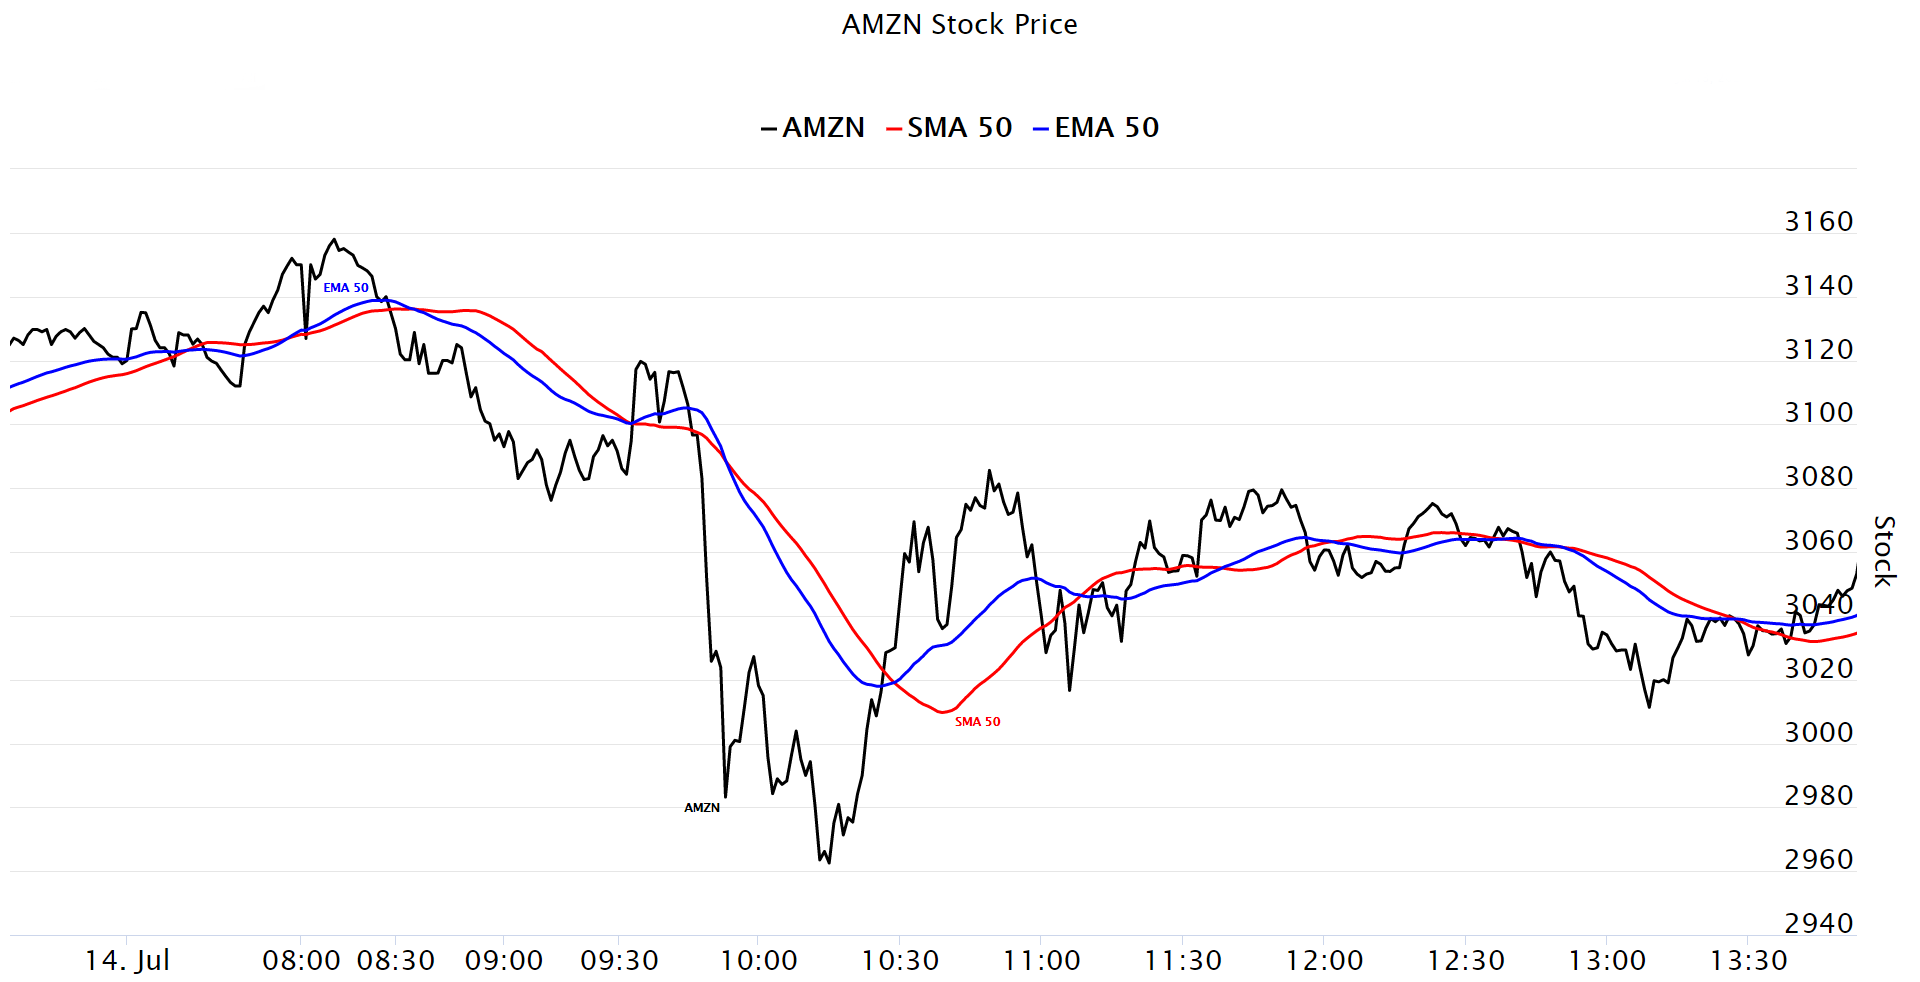
\includegraphics[scale=0.22]{images/emasma.png}
\caption{Az EMA és az SMA átlagok összevetése.}
\label{fig:emasma}
\end{figure}
\noindent Mint az látható, az EMA gyorsabban reagál a részvény mozgására, mint az ugyanolyan periódusú SMA. Azonban az EMA-t nem ebben a formában fogom hasznosítani, hanem egy következő indikátor számításához fogom felhasználni, amit a következő alfejezetben foglalok össze.
\newpage

\Section{Moving Average Convergence/Divergence\\(MACD)}

Az MACD egy egyszerű és megbízható trend követő indikátor, mely két mozgóátlag közötti kapcsolatot mutatja meg. Az MACD-t úgy számítjuk ki, hogy a 26 periódusú EMA-t kivonjuk a 12 periódusú EMA-ból, és ennek a két mozgóátlagnak a különbsége adja az MACD vonalat, melyhez egy szignál vonalat is szoktak társítani. Az MACD egy nulla alatt és fölött ingadozó függvény minimum és maximum határ nélkül. A szignál vonal a 9 periódusú EMA-ja az MACD-nek, tehát
\begin{align*}
\text{MACD} &= \text{EMA}_{12}(\text{záróár}) - \text{EMA}_{26}(\text{záróár}), \\
\text{Szignál} &= \text{EMA}_9(\text{MACD}).
\end{align*}
A szignál vonal arra való, hogy jelezze a vásárlási és eladási pontokat. Többféleképp értelmezhetjük a függvények mozgását, de a leggyakoribb alakzatok, amit figyelnek a keresztezések, a divergenciák és a hirtelen mozgások.
\begin{figure}[ht]
\centering
\includegraphics[width=\textwidth]{images/macd.png}
\caption{Az MACD és a szignál függvény grafikonja.}
\label{fig:macd}
\end{figure}

\noindent A képen látható, ha a 12 periódusú a 26 periódusú felett van, akkor az MACD is a 0 érték fölött mozog, s minél magasabb az MACD értéke, annál nagyobb a két mozgóátlag közötti távolság is. Az MACD és a szignálja, ha keresztezik egymást, akkor ezt egy jelzésnek tekintjük. Amennyiben a szignál felülről keresztezi a MACD vonalát, akkor ezt vásárlási, ha alulról, akkor eladási jelzésként értelmezhetjük.

\Section{Relative Strength Index (RSI)}
Az RSI egy nagyon népszerű momentum indikátor, mely az árváltozásokat figyeli, és ezáltal megállapíthatóak a túlvett és túladott állapotok. Az RSI az MACD-hez hasonlóan egy oszcillátor, mely két határértékkel rendelkezik: 0 és 100 között mozog az értéke. Hagyományosan 70-től felfelé azt mondjuk, hogy a részvény túlvett és várhatóan visszafordul a trend, 30 alatt pedig túladott, alulértékelt. Ezt a két szintet szokás jelzésként használni. Számítását tekintve az előzőekhez képest összetettebb, két részben érdemes nézni.
\begin{align*}
1) \hspace*{2mm} \text{RSI} &= 100 - \left[\frac{100}{1+\frac{\text{Average Gain}}{\text{Average Loss}}}\right], \\
2) \hspace*{2mm} \text{RSI} &= 100 - \left[ \frac{100}{1+\frac{(\text{Previous Average Gain}*(\text{period}-1)) + \text{Current Gain}}{(\text{Previous Average Loss} * (\text{period}-1)) + \text{Current Loss}}} \right].
\end{align*}

\begin{figure}[ht]
\centering
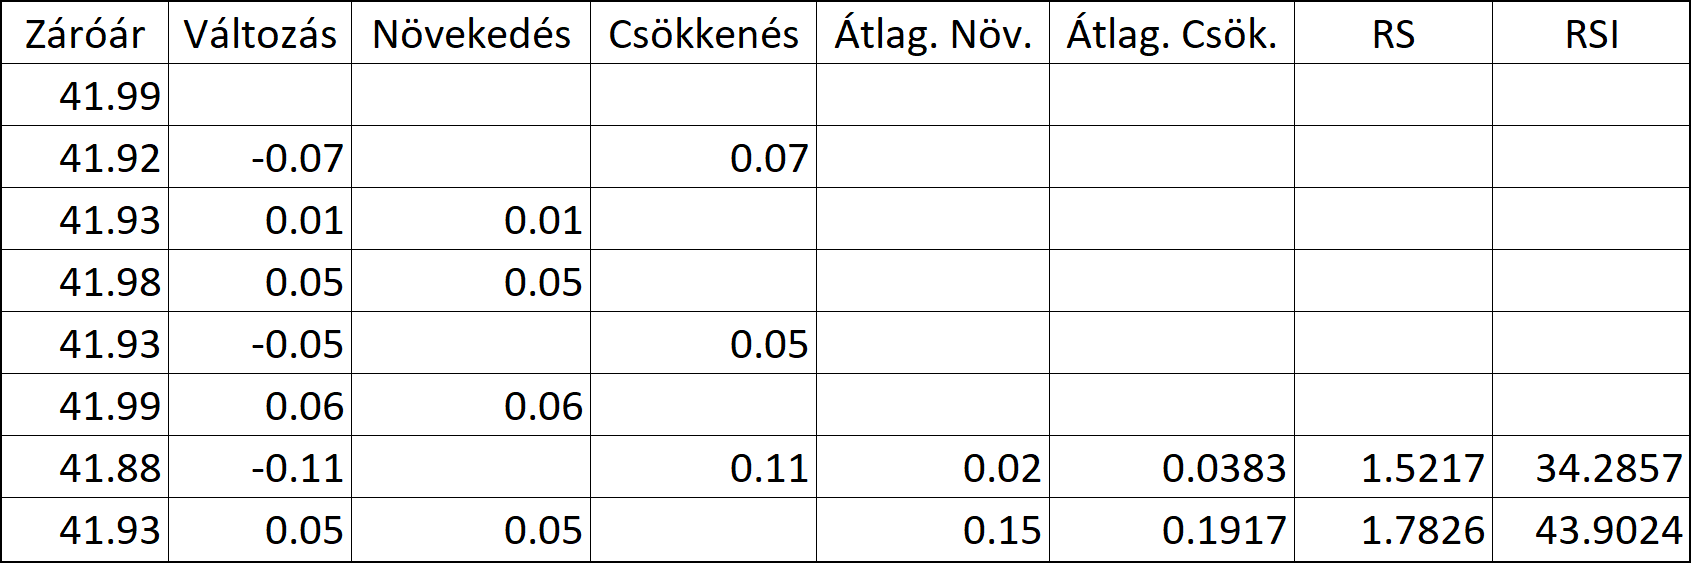
\includegraphics[scale=0.25]{images/RSI_calc.png}
\caption{Példa az RSI indikátor számítására.}
\label{fig:rsicalc}
\end{figure}
\noindent Tekintsük a fenti példa táblázatot, melyre az $\text{RSI}_6$-ot végeztem el. Az első lépésben kiszámítom a 6 napos átlagát a Növekedés oszlop, majd a Csökkenés oszlop elemeinek a második elemtől fogva. E kettő hányadosa adja az RS értéket. Majd az első képletbe behelyettesítve kapom az RSI értékét.
A következő átlagokat már a második képlet alapján kell kiszámítani úgy, hogy az előző sor átlagait megszorozzuk öttel, s hozzáadjuk a jelenlegi sorban található növedesést/csökkenést attól függően, hogy merre mozdult el a részvény ára.

\begin{figure}[ht]
\centering
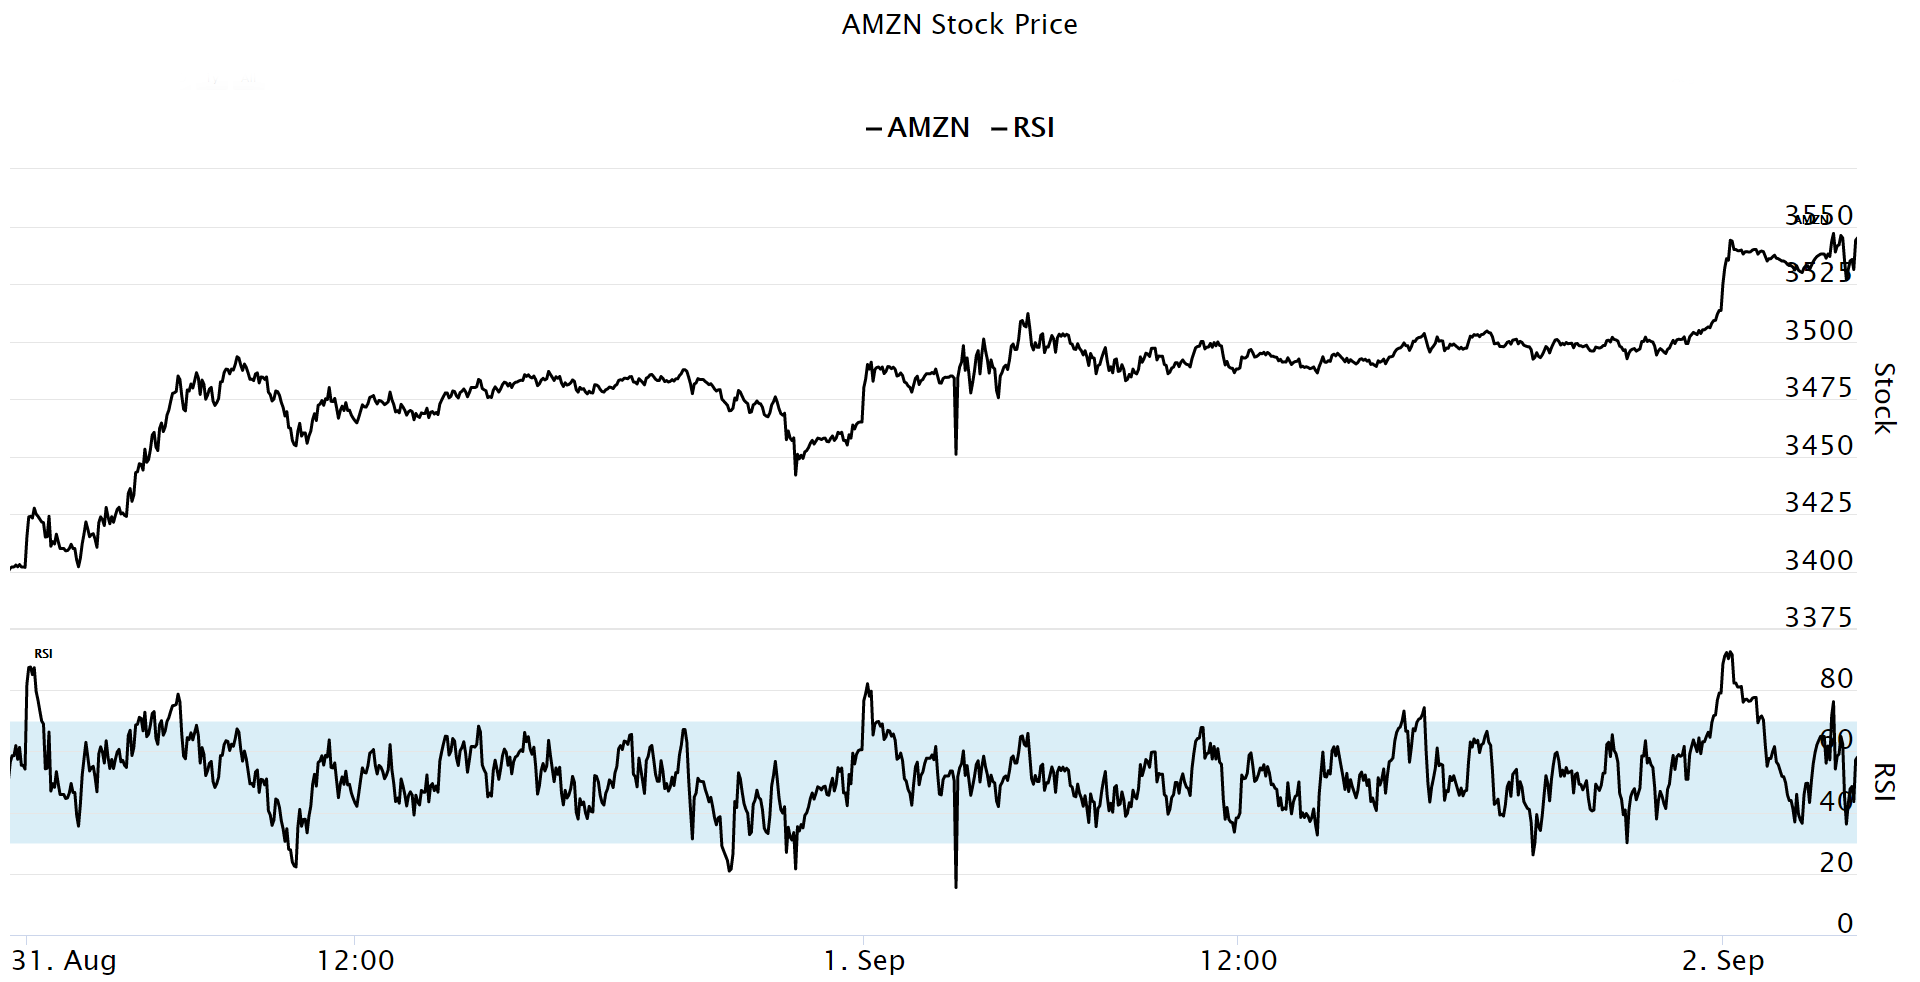
\includegraphics[width=\textwidth]{images/RSI.png}
\caption{Az RSI indikátor mozgása az árfolyammal együtt.}
\label{fig:rsi}
\end{figure}
\noindent Néhány elemző azonban nem a fent említett szinteket alkalmazza, hanem a középvonal keresztezést nézik. Más szavakkal, ha az RSI nagyobb, mint 50, akkor pozitív jelzésnek, ha kisebb, mint 50, akkor negatív jelzésnek tekintik.

Ha tekintjük a \ref{fig:rsi}-as ábrát, akkor azt láthatjuk, hogy több alkalommal jelzett az RSI indikátor. Amikor volt egy nagyobb esés, akkor túladott jelzést mutatott az indikátor, amikor pedig hirtelen ugrások voltak az árfolyamban felfelé, akkor túlvett jelzést kaptunk. Ha az első túlvett jelzést megnézzük, akkor valóban lehetett volna profitot szerezni, azonban ha tovább haladunk a grafikonon akkor látható, hogy az árfolyam nem állt meg, további emelkedést mutatott. Ezért is érdemes az indikátorokat megerősíteni több másik indikátorral.

\Section{Indikátorok vizsgálata}
A fent részletezett indikátorokat érdemes górcső alá vetni, s a hatékonyságukat vizsgálni. Az indikátorok feltételeit felhasználva mértem a jelzések számát, illetve, hogy hány esetben növekedett az árfolyam 5, illetve 10\%-al, s a hatékonyságukat 0-100-ig tartó skálán pontoztam. Az általam összegyűjtött 44 darab vállalatra lefuttattam a mérést és összegyűjtöttem ezeket egy táblázatban.
\begin{figure}[ht]
\centering
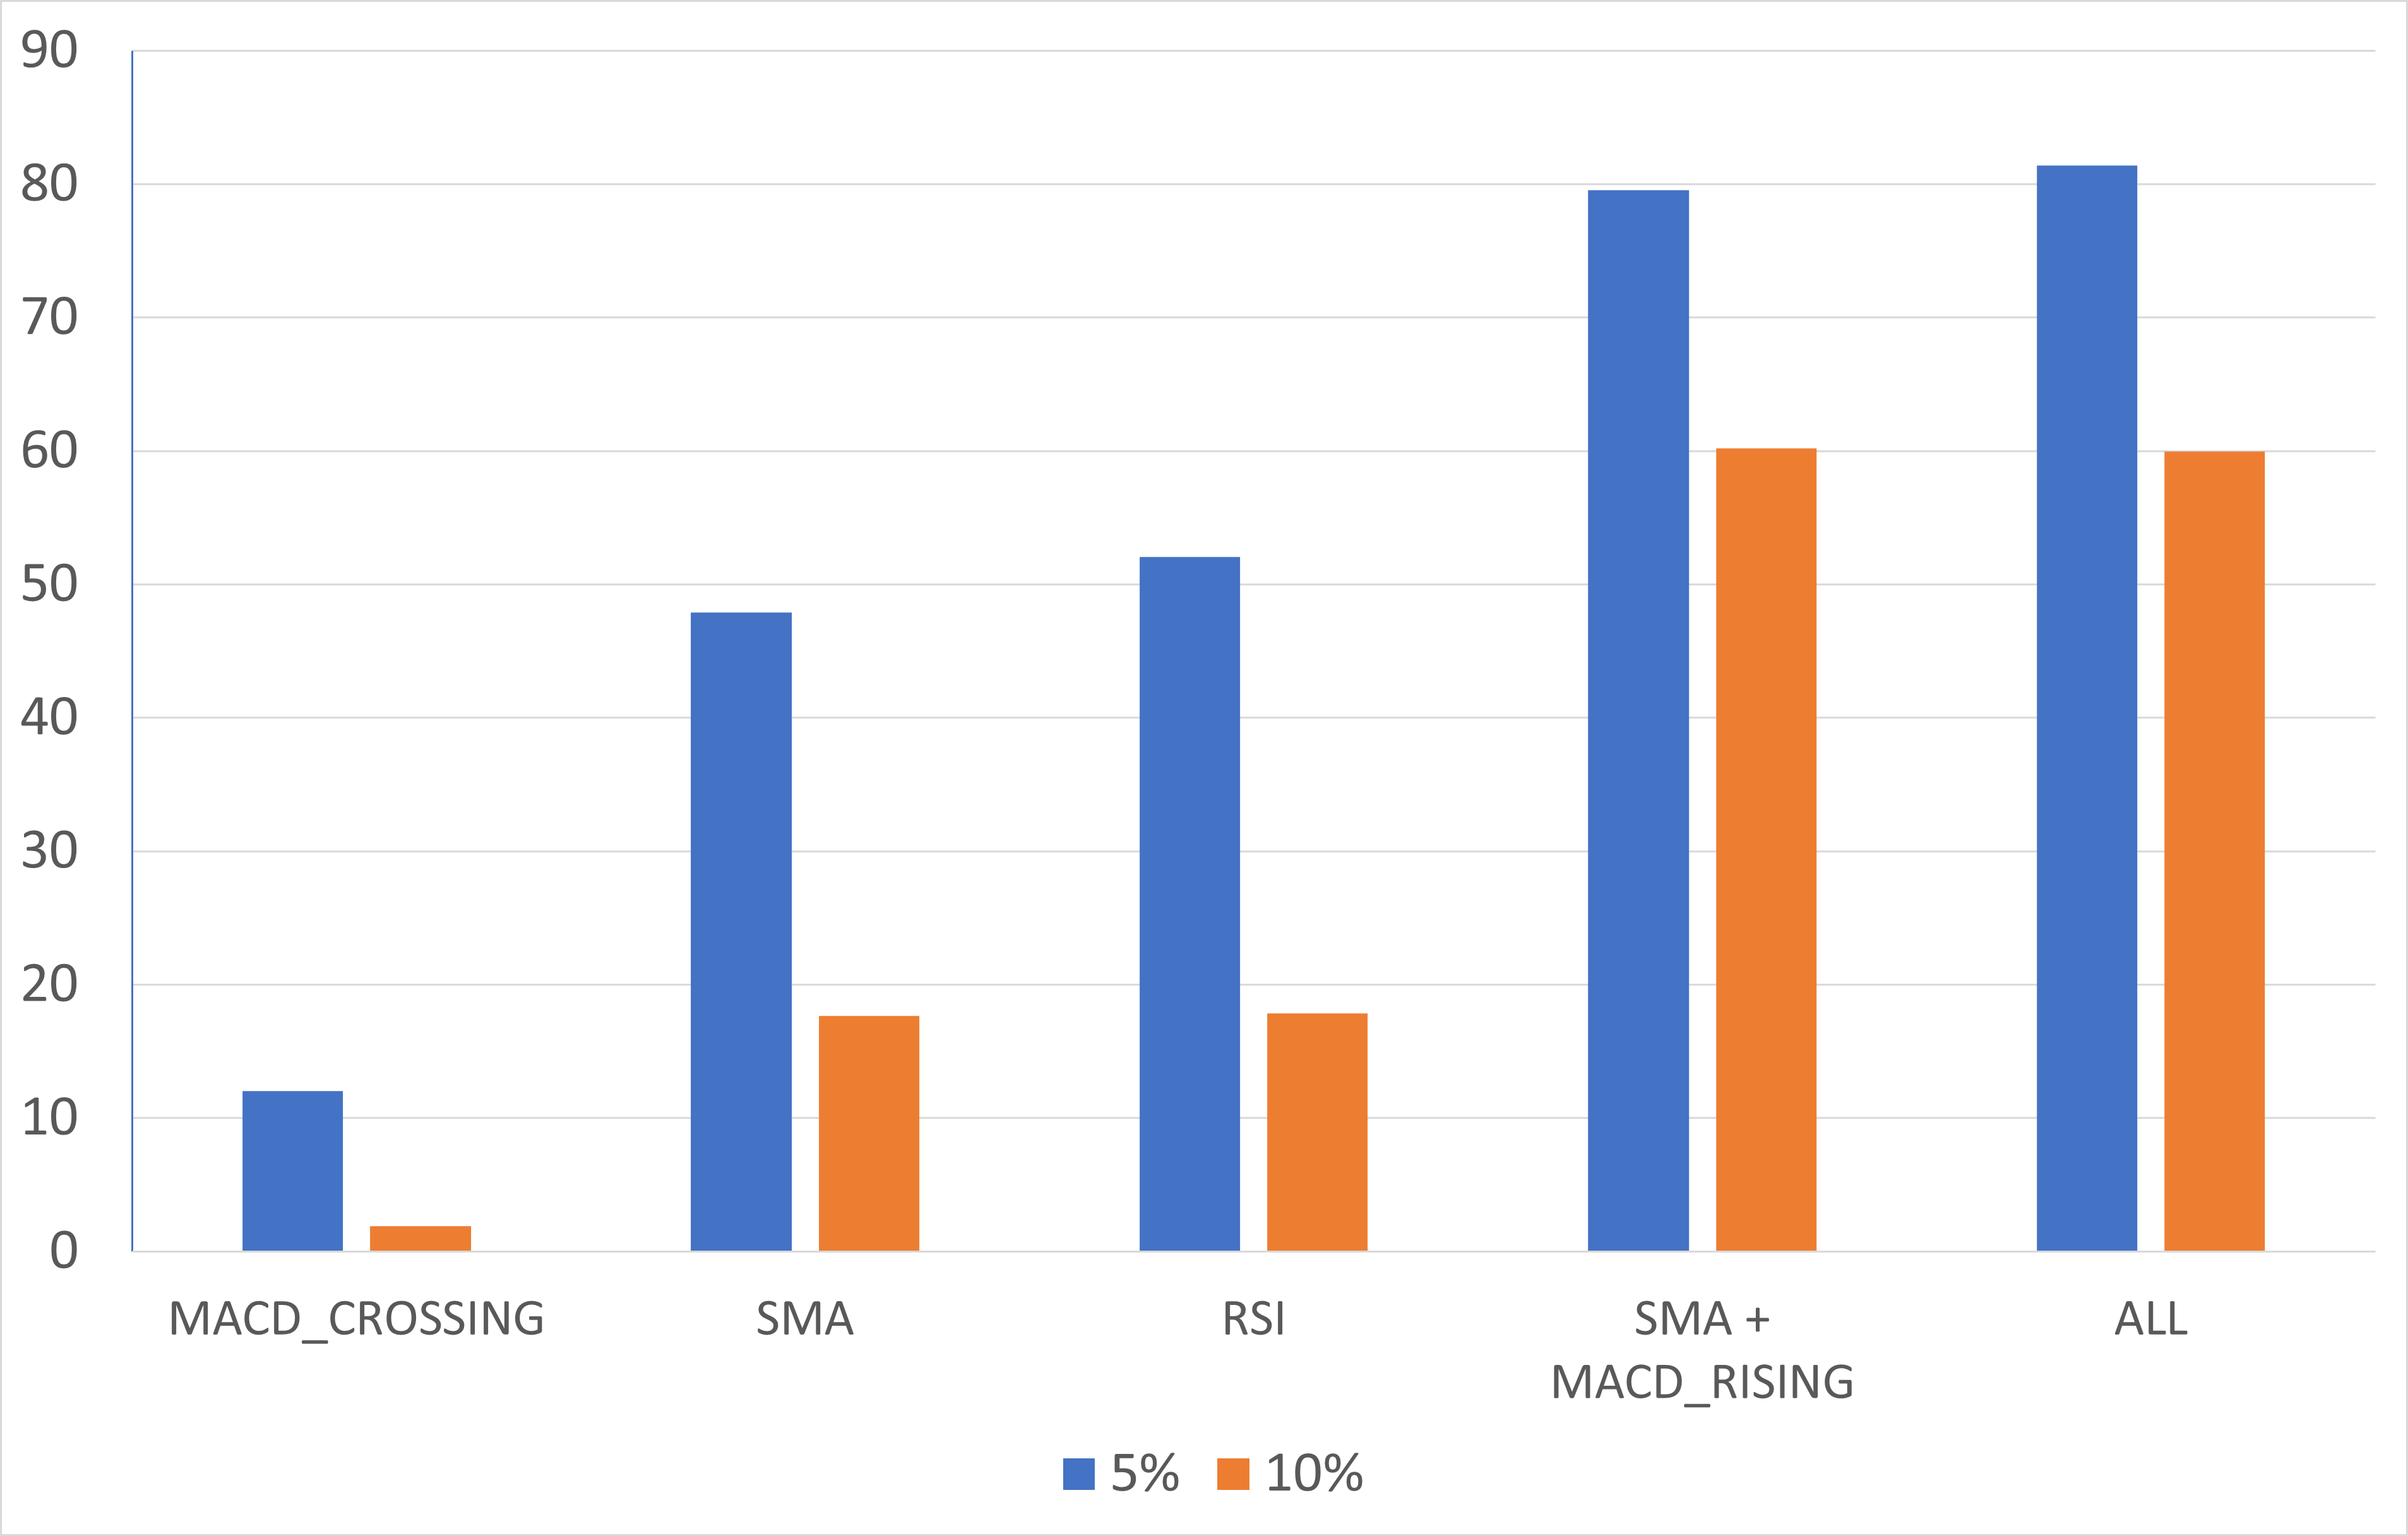
\includegraphics[scale=0.35]{images/indicator_test.png}
\caption{Az indikátorok hatékonyságának mérése.}
\label{fig:indicator_test}
\end{figure}

\noindent A fenti ábráról az olvasható le, hogy önmagukban az indikátorok nem annyira hatékonyak, ezért érdemes őket csoportosan nézni. Ha megnézzük az első mérést, amely az MACD és a szignál függvényének keresztezését figyeli, akkor azt mondhatjuk el, hogy 5\%-os emelkedésben kicsit alulteljesít, azonban a 10\%-osban nagyon lemarad a többitől. Az RSI és az SMA közel egy szinten vannak, azonban ha elkezdjük őket keresztezni, akkor közel 30\%-os emelkedést tapasztalhatunk. Ez abból fakad, hogy az ÉS kapcsolat szigorúbb feltételeket állít, ezért kevesebb lesz a jelzések száma.

Az indikátorokkal az a legnagyobb probléma, hogy mire jeleznek az indikátorok, addigra már az árfolyam rég elindult pozitív vagy negatív irányba. Emiatt sosem fogjuk tudni a legjobb áron megvenni, illetve eladni a részvényt, ezért nagyon fontos a jelzések pontosítása.
\begin{figure}[ht]
\centering
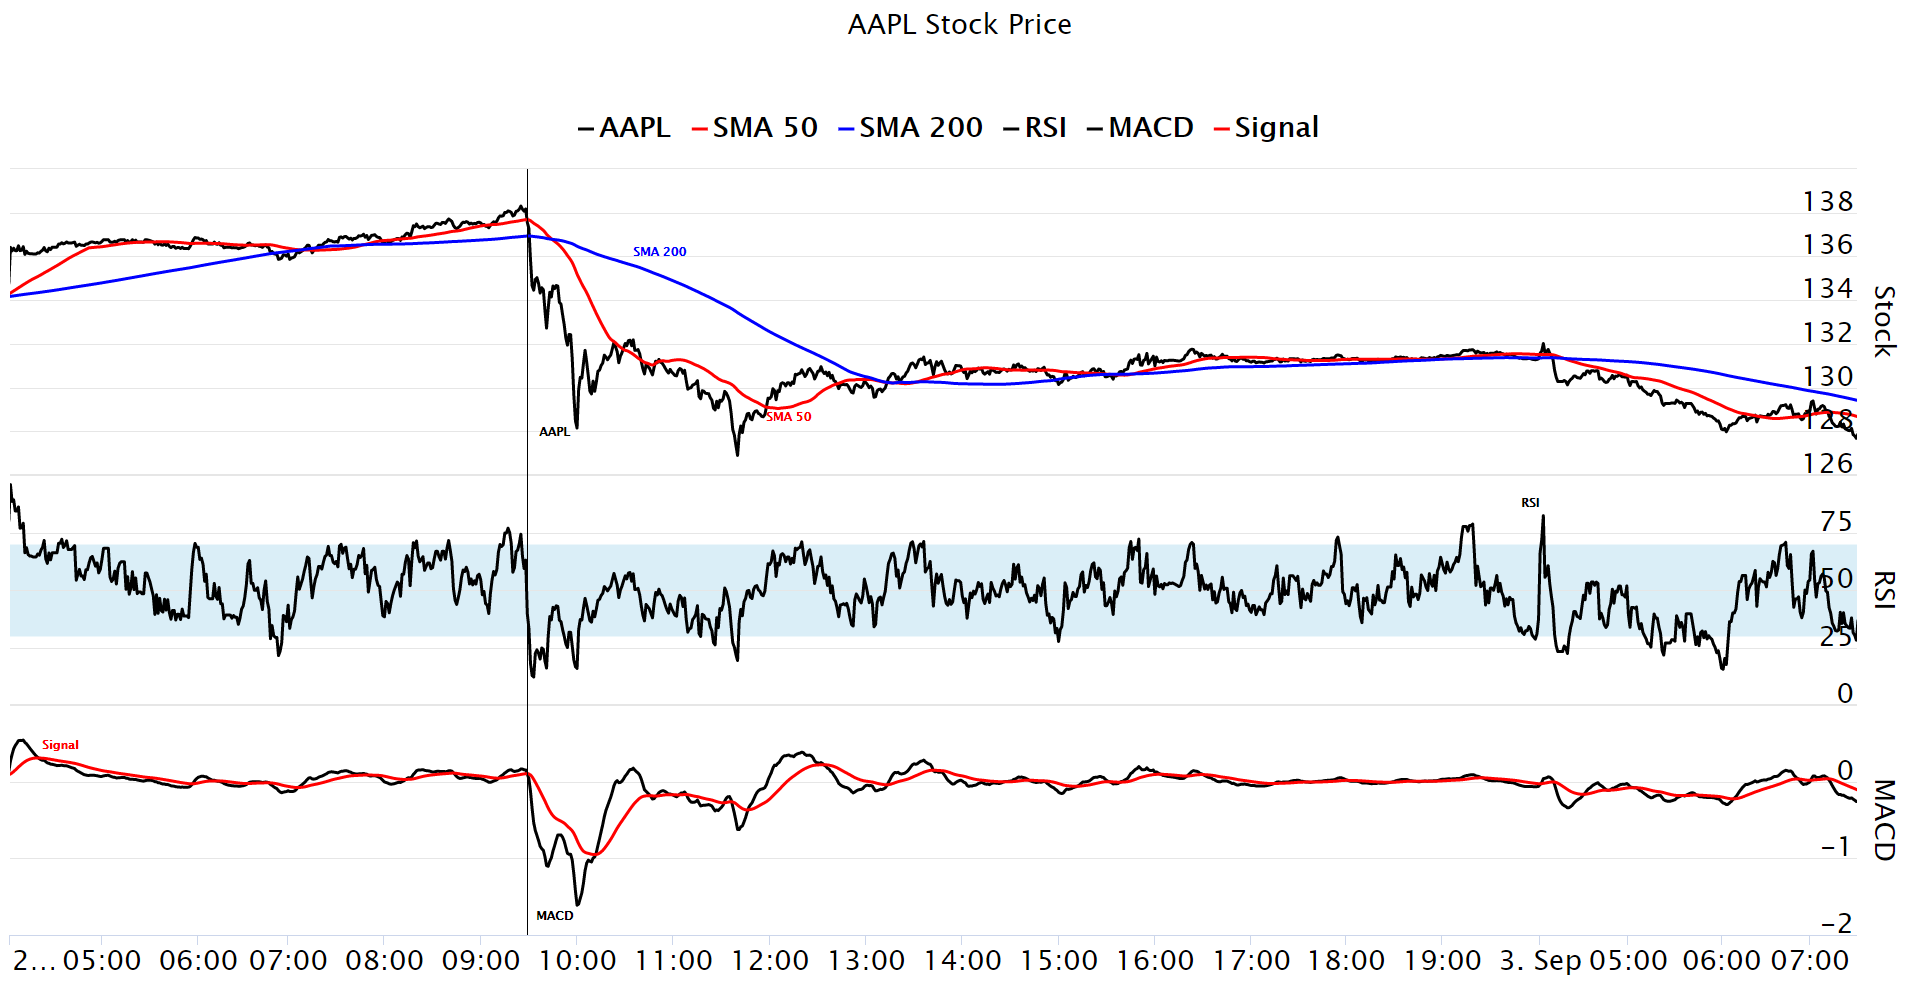
\includegraphics[width=\textwidth]{images/indicator_error.png}
\caption{A jelzések késése az Apple részvényén.}
\label{fig:indicator_error}
\end{figure}
\newpage
\Section{Részvény shortolása}
A kereskedők minden lehetőséget megfognak ahhoz, hogy profitot tudjanak termelni maguknak. A következő technika, amit alkalmaznak is besorolható az árfolyamnyereséges kategóriába, azonban az indikátorokra tett hatása miatt külön dolgozom fel. A piacon lehetőség van arra, hogy kölcsön kérjenek részvényeket befektetők annak reményében, hogy az árfolyam csökkenni fog. Amikor megszerezte a részvényeket eladja, és amikor csökkenésnek indul a részvény kivárja a megfelelő időpontot, és utána visszavásárolja őket, majd visszaadja a részvényeket az eredeti tulajdonosának. Így a kereskedő a különbséget profitként könyveli el, ebből persze lejönnek a költségei a tranzakciónak, illetve bérlési költséget is felszámolnak érte. Ezt a folyamatot shortolásnak nevezik.
\begin{figure}[ht]
\centering
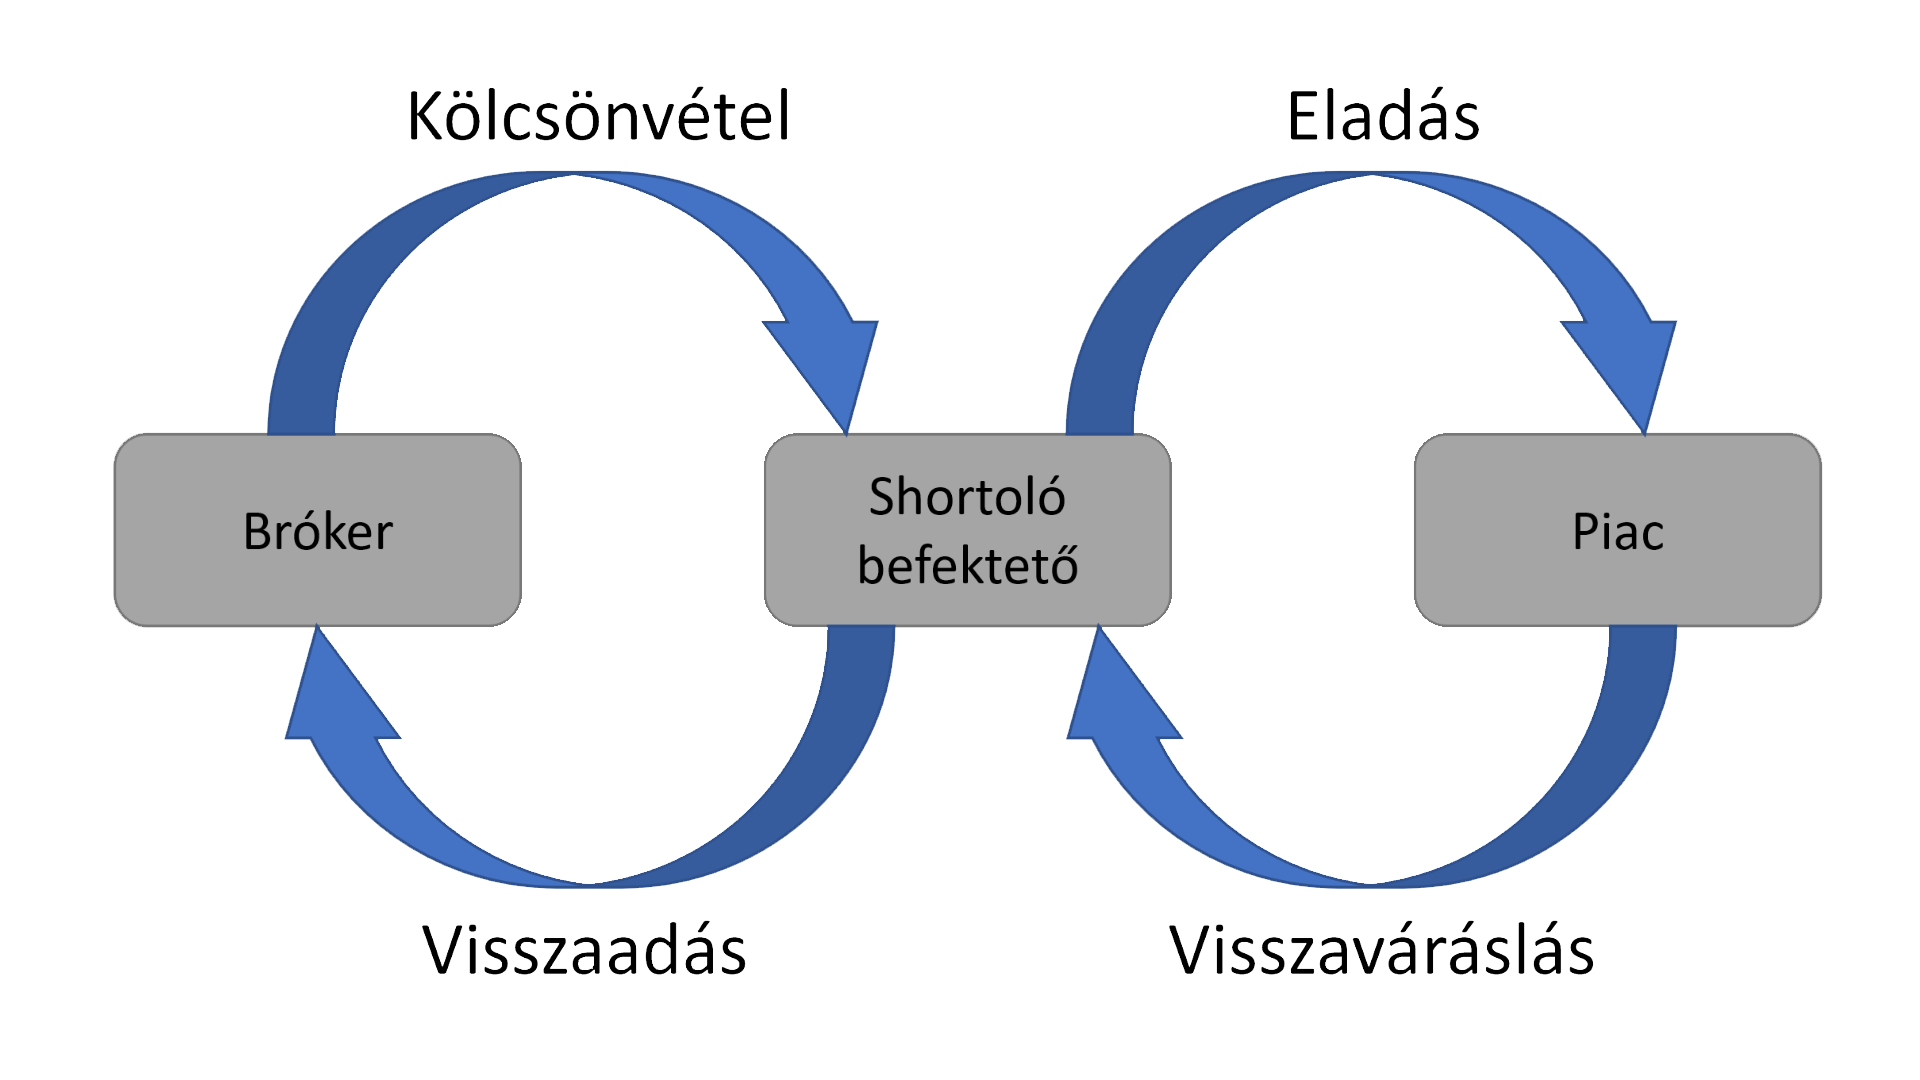
\includegraphics[scale=0.20]{images/short.png}
\caption{A shortolás folyamatának ábrája.}
\label{fig:short}
\end{figure}

\subsection{Short squeeze}
A short squeeze egy részvény értékének meredek emelkedése, amely elsősorban a részvények túlzott shortolásából adódik. Akkor következik be, amikor a részvények iránti kereslet túl nagy, a kínálat pedig túl kevés. Amikor a kereskedők elképzelésével ellentétes irányba, azaz felfelé mozdul el a részvény árfolyama, akkor, hogy csökkentsék a veszteségeiket elkezdik visszavásárolni a részvényeket. Amikor visszavásárolják a részvényeiket, akkor megemelkedik a részvény ára, ezzel még több shortoló befektető kényszerül visszavásárolni a részvényeit. A short squeeze általában azoknál a részvényeknél szokott előfordulni, ahol magas a bérleti költség, hiszen ez még nagyobb nyomást helyez a befektetőkre, hogy a pozíciójukat fedezzék.
\begin{figure}[ht]
\centering
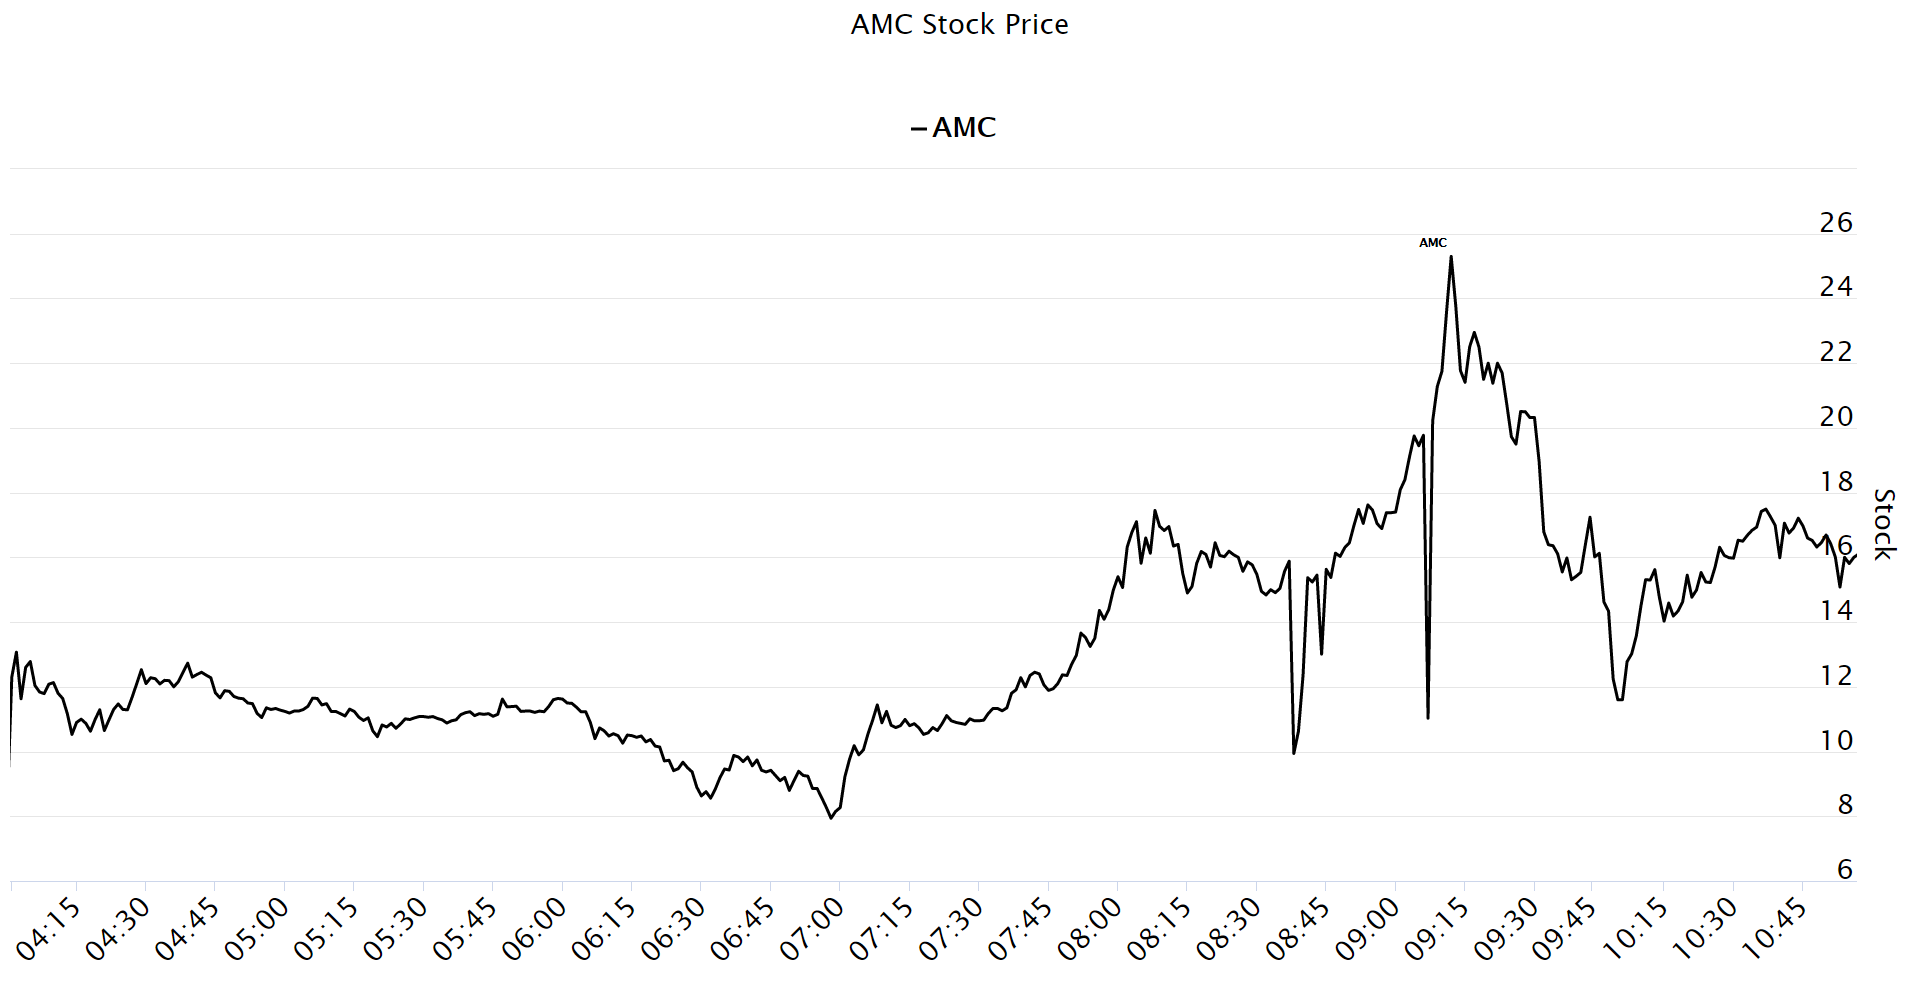
\includegraphics[width=\textwidth]{images/short_squeeze.png}
\caption{Short squeeze: 5 perc alatt 230\%-os emelkedés az AMC részvényén}
\label{fig:short_sq}
\end{figure}

\Section{A kriptovaluta}
A napjaink egyik felkapott témája a kriptovaluta. Ezt az is mutatja, hogy már több mint ezer kriptovaluta közül választhatunk. A leghíresebb kétségek nélkül a Bitcoin, amely a szakdolgozat írásának pillanatában 55 000 $\pm$ 5 000\$-ért vásárolható meg. Mi is az a kriptovaluta? A kriptovaluta egy digitális pénznem, amelyet kriptográfiai módszerrel védenek, így közel lehetetlen a hamisítása. A blokklánc (blockchain) technológia tartja fent ezt a védelmet, amelyet egy példán keresztül mutatnék be.

\begin{figure}[ht]
\centering
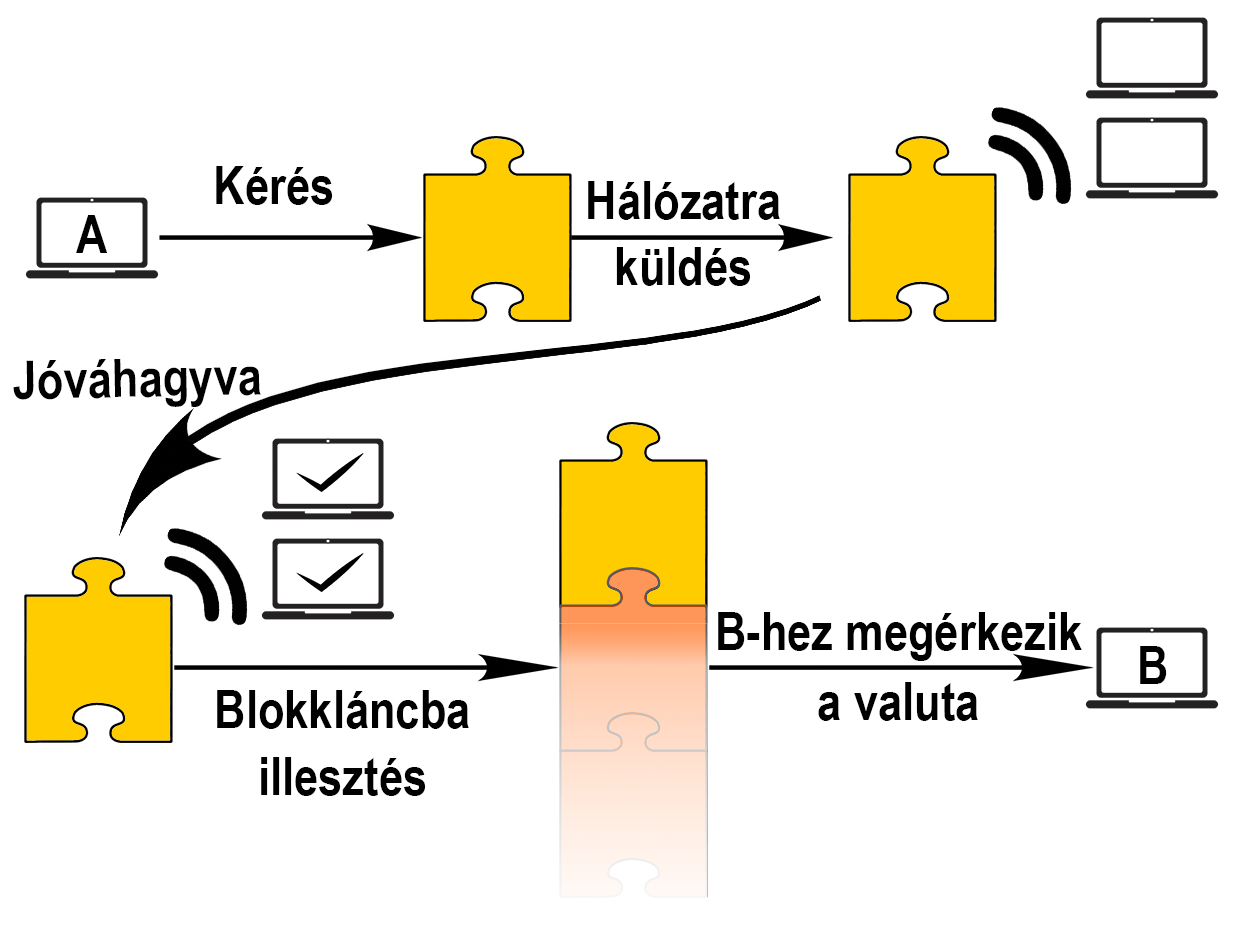
\includegraphics[scale=0.22]{images/krypto.png}
\caption{Tranzakció végrehajtása blokklánc technológiával.}
\label{fig:krypto}
\end{figure}

Tegyük fel, hogy kriptovalutát szeretne küldeni az \textbf{A}-val jelölt személy a \textbf{B}-vel jelölt személynek. \textbf{A} egy kérésben jelzi a szándékát, mely egy blokkba kerül beillesztésre. Egy blokk 1MB maximálisan, amely több mint 500 tranzakciót jelent. Ez a blokk minden résztvevő számára közvetítésre kerül, ők fogják validálni a tranzakciókat, és ha jóváhagyták, akkor a blokklánc végére illesztik a blokkot, ami ettől fogva kitörölhetetlen, hiszen akkor megváltozna a hash értéke, és a többi résztvevő visszadobná a blokkot. Ekkor már vége is van egy tranzakció feldolgozásának, átkerült a kívánt összeg a \textbf{B} számlájára.
Tehát látható, hogy a hálózat védelme egészen hatásos, de miért éri meg bárkinek, hogy egy kriptovaluta tranzakcióit, integritását óvja?

\subsection{A kriptovaluta bányászata}
A kriptovaluta bányászatán azt értjük, hogy a számítógépünket a kriptovaluta hálózathoz kapcsoljuk és a blokkok vizsgálatát végezzük el. Ez egy automatikus folyamat, csupán egy programot kell hozzá elindítani. A számításokhoz a videókártyát használják, hiszen ezzel a leggyorsabb elvégezni a matematikai képleteket. A Bitcoin úgy lett tervezve, hogy a blokkok 10 percenként érkeznek, és ha sikerül megoldani a hashelést, akkor a hozzáadott számítási kapacitás alapján szétosztásra kerül 6.25 BTC, amely körülbelül 105 millió forint értékű. Hogy minél nagyobb számítási kapacitást érjenek el egyre több videókártyát vásárolnak a bányászok, emiatt a készlet lecsökken, és az áruk is az egekbe emelkedik.

\begin{figure}[ht]
\centering
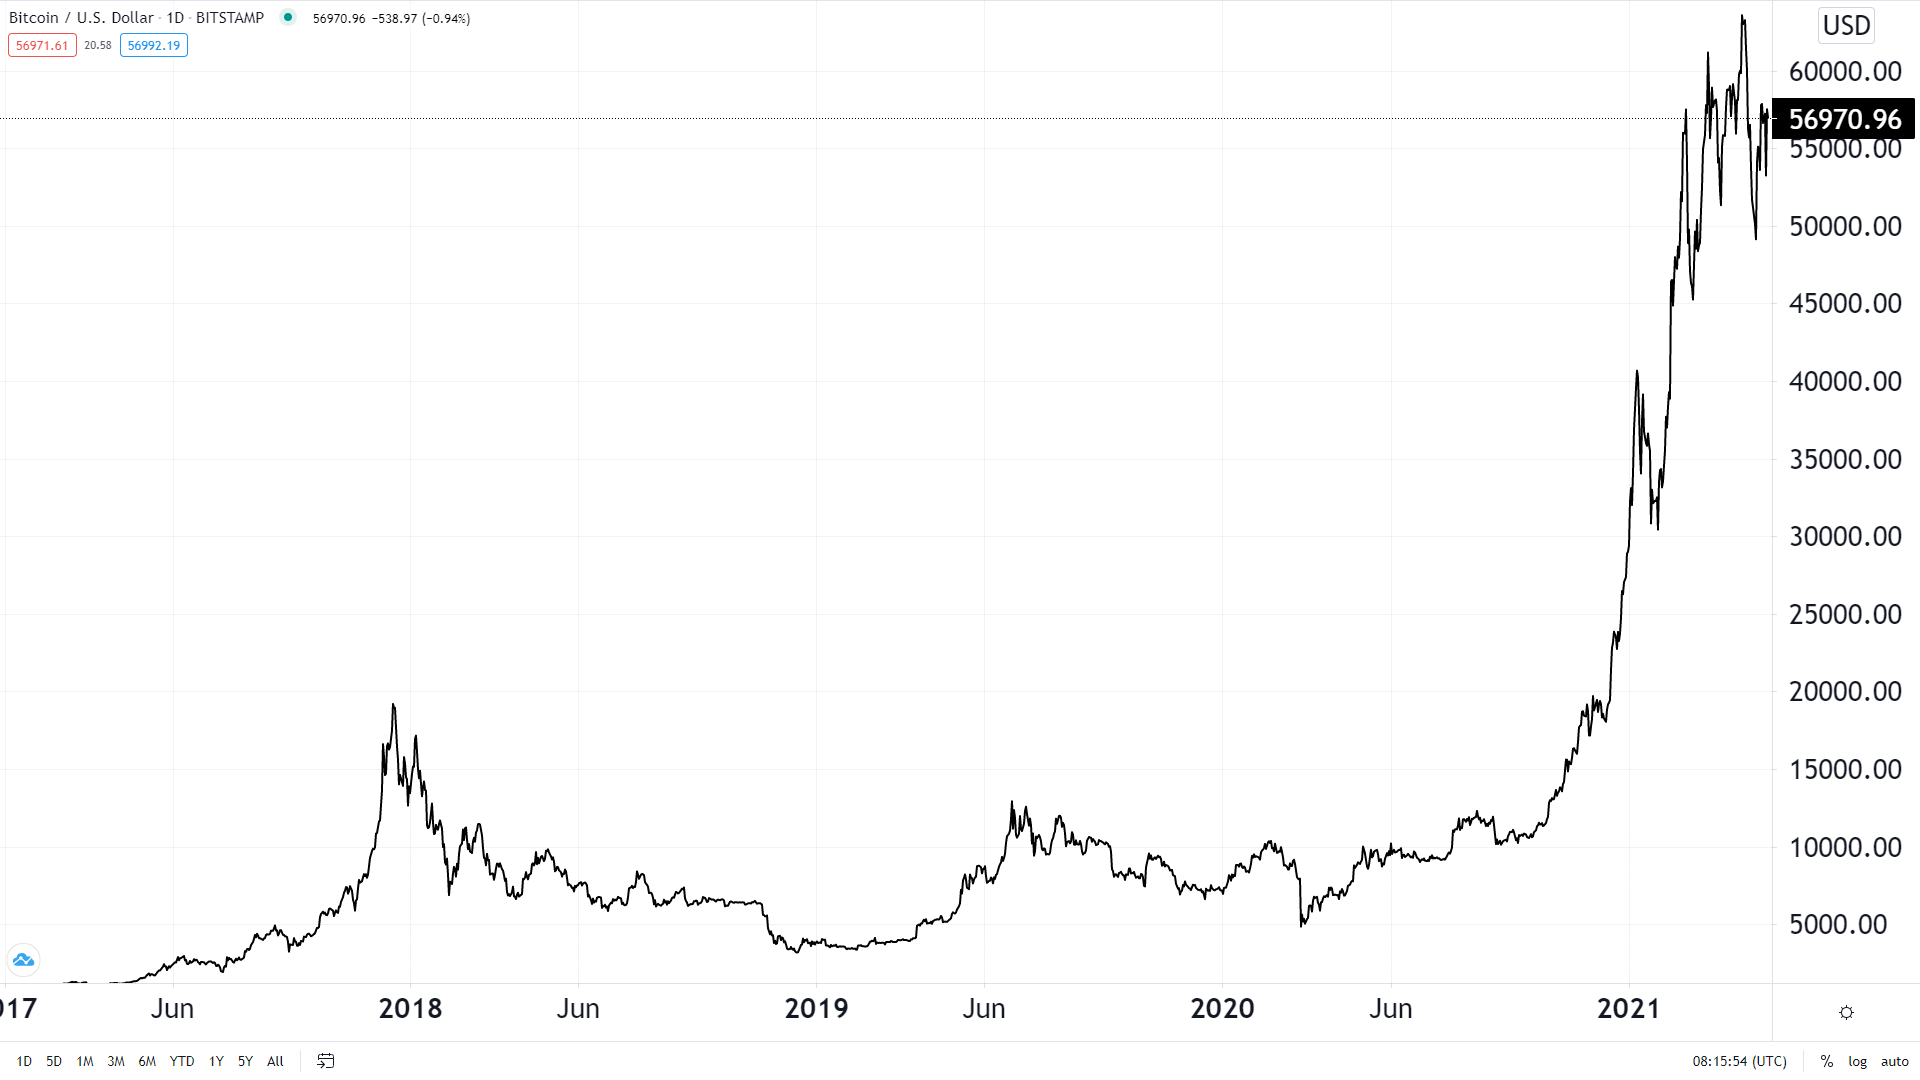
\includegraphics[width=\textwidth]{images/BTC.png}
\caption{A Bitcoin árfolyamának alakulása \cite{Tradingview}.}
\label{fig:BTC}
\end{figure} 